

\begin{frame}
	\frametitle{History}
	\begin{center}
		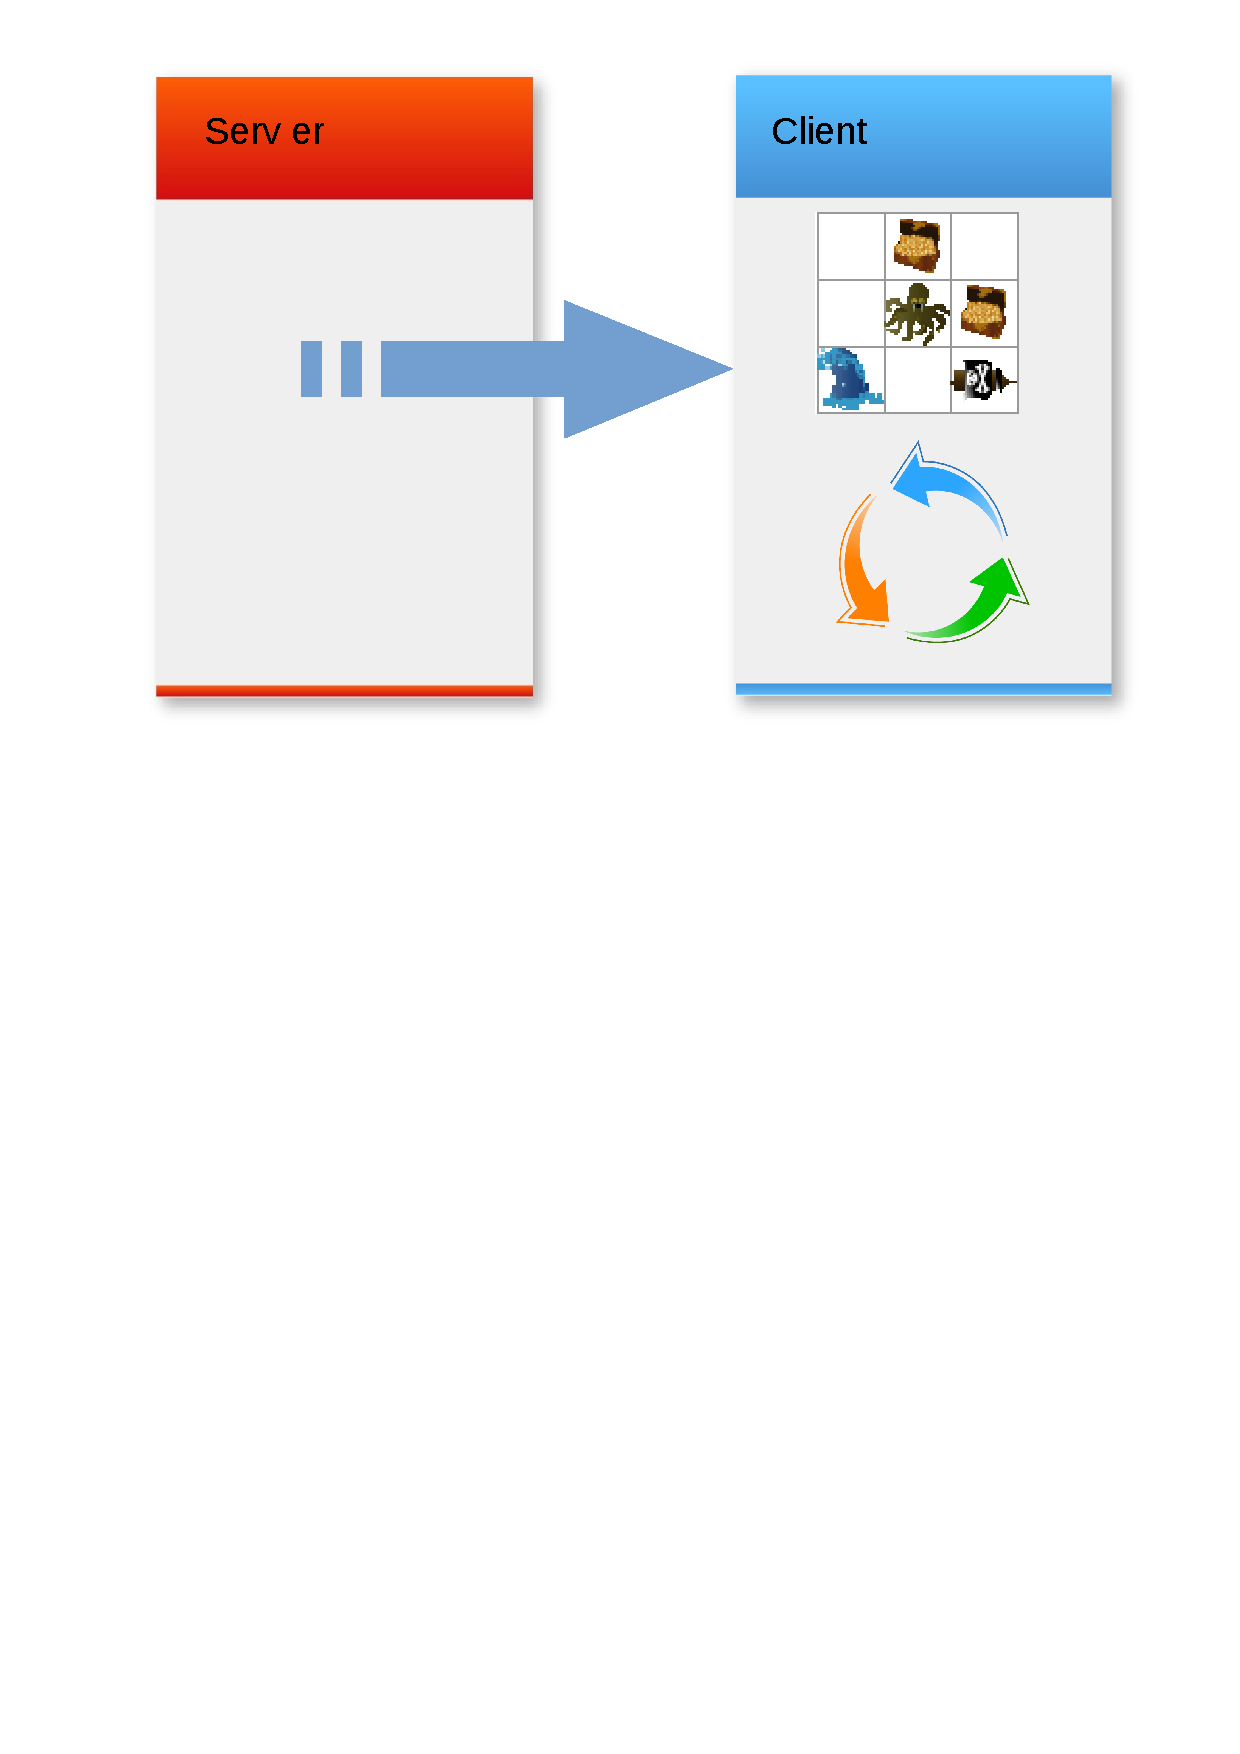
\includegraphics[scale=0.5]{simulation/history1.pdf}
	\end{center}
	%Wir haben ganz am Anfang ohne VM angefangen. Es gab zwei Ansätze, endweder die Simulation etc. auf dem Server oder auf dem Client. Der erste Entwurf sah vor, dass wir auf dem Client den eingegebenen Code zu Javascript compilieren und dann auf dem Client simulieren. Es traten viele Probleme mit dem compilieren auf, also entschlossen wir uns recht früh für eine VM.
\end{frame}

\begin{frame}
	\frametitle{History}
	\begin{center}
		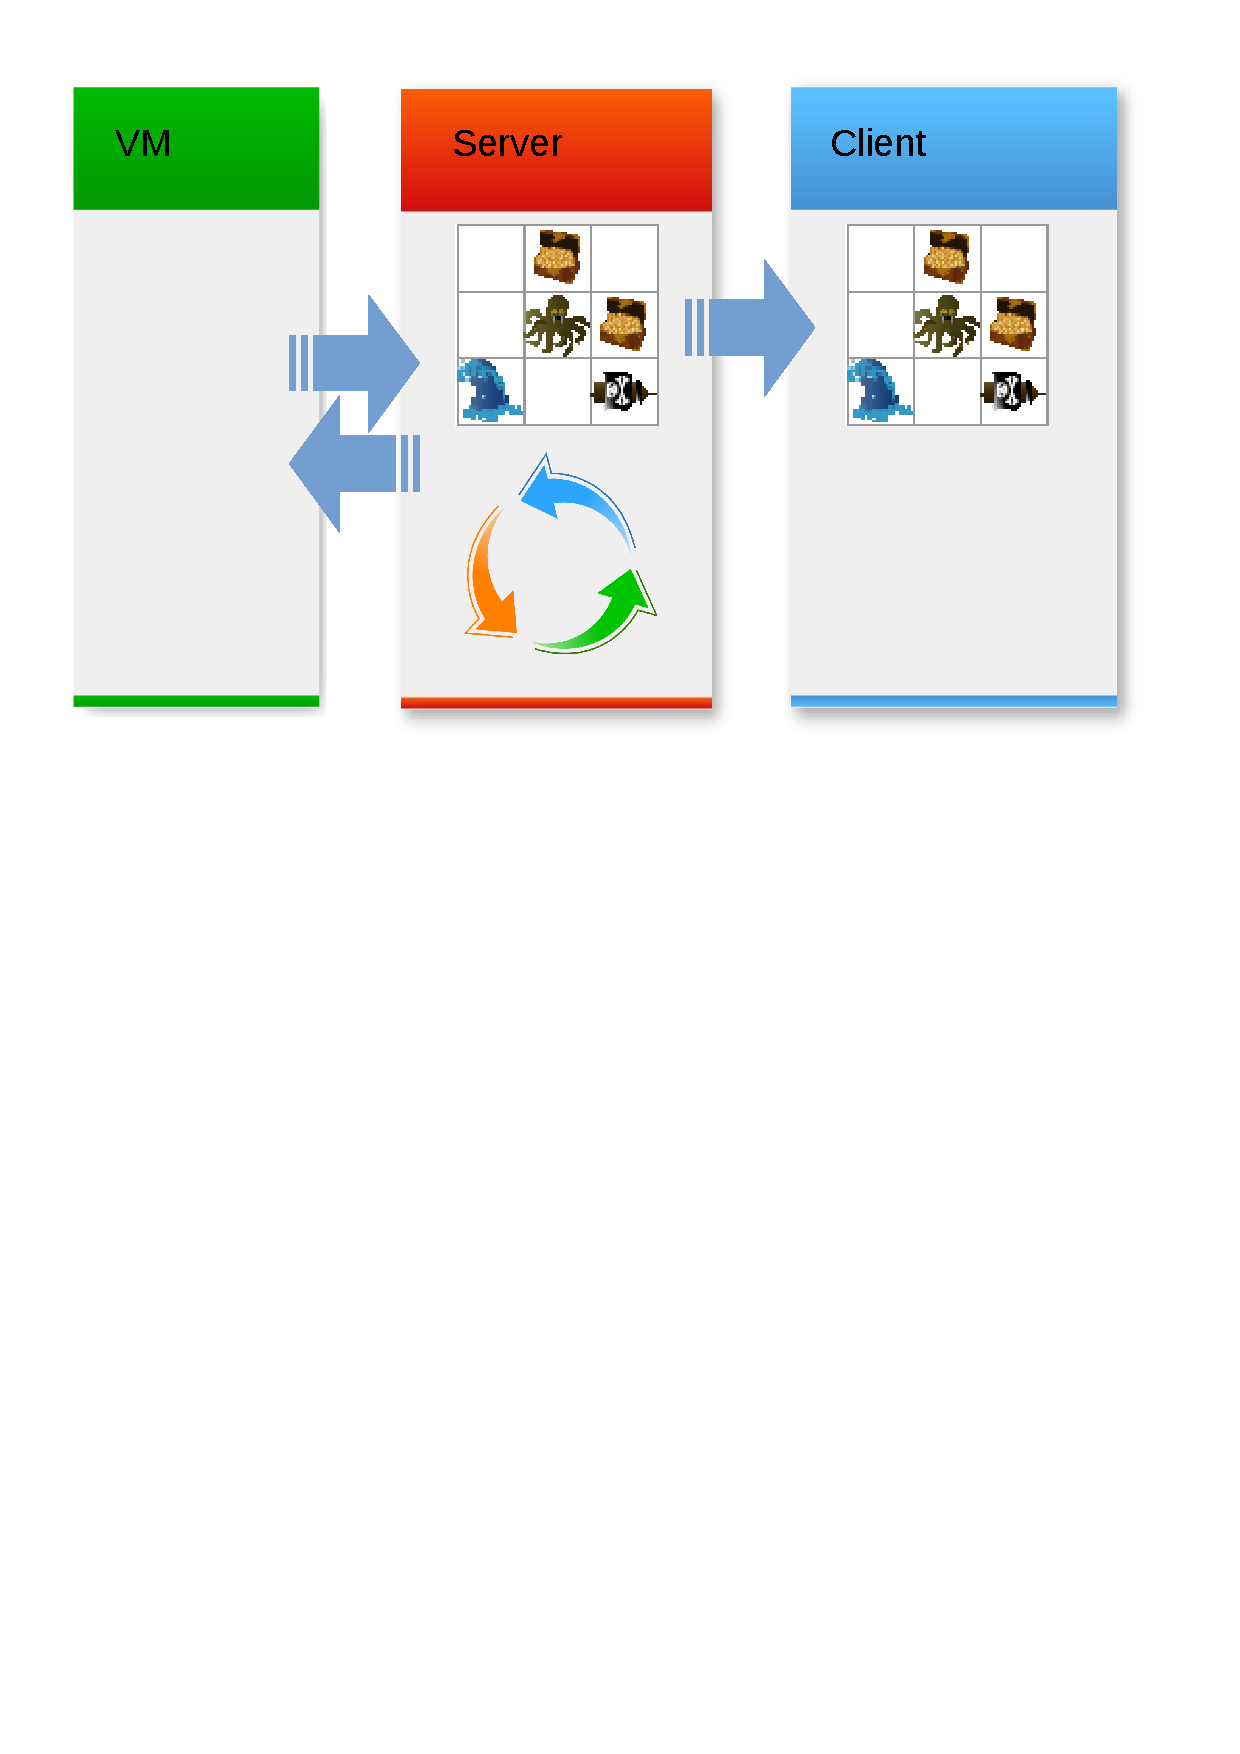
\includegraphics[scale=0.5]{simulation/history2.pdf}
	\end{center}
	%Am Anfang leitete der Server die Ausgaben der VM nur an den Client weiter, dies funktionierte prima, bis wir an den Punkt kamen, dass die VM auch Anfragen stellen konnte und dann wurde es sehr unpraktisch, immer auf Antwort vom Client zu warten. Wir haben das jetzt so gelöst, dass die Simulation quasi komplett auf dem Server läuft und nur die Änderungen des Grids an den Client weitergegeben werden.
\end{frame}
